\documentclass[11pt]{report}
\usepackage{fullpage}
\usepackage{graphicx}
\usepackage{float}
\restylefloat{table}
\begin{document}

\title{Developing a tool to increasing perception and understanding of Autism}
\author{Ashley Peacock}
\maketitle

\textbf{Abstract}\\
--add this when i'm finished 

\begin{quote}
"if you deal with 'challenging behaviours' in autism, do not focus on the iceberg; do understand the underlying causes of the behaviours and try to develop an approach not based on symptoms but on prevention. Challenging behaviours are caused by problems of communication, social understanding, by different imagination, by sensory problems...Therefore try to understand autism 'from within'. It is easier said than done, because it requires an enormous effort of imagination: we need t learn to put ourselves in the brains of autistic people and then we will understand better through their eyes the obstacles in their attempts to survive among us" - Theo Peeters \cite{olgab}
\end{quote}

\tableofcontents

\chapter{Introduction}

The projected started by firstly creating and considering various project proposals that may benefit people with ADHD or Autism. Following this, research and feedback aided the selection of the project an "Autism Simulator" whereby the user plays as a child with Autism and gets to experience some of the difficulties, specifically sensory related difficulties through their eyes. Interviews were conducted with people on the Autistic spectrum, professionals and school teachers as to inform this choice and give further clarity of the challenges faced as well as consultation from the LAER group. Following goal selection, a prototype of the simulator was created using a Game Engine for speedy development and evaluated by the LAER group with an additional evaluation in the form of an on-line survey where participants were able to view a video demo of the simulator and give feedback. The first playable version was subsequently created after an extensive re-write of the system due to performance issues and then evaluated by various students as a formative evaluation to aid game-play decisions and improvements before a summative evaluation was completed by various members of the university involved in education. 

\section{Selecting a project}
The project started with the purpose of creating software to benefit someone with Autism, ADHD or those in contact with these conditions such as family members or carers. Both Autism and ADHD are developmental disorders that start from birth and affect the individual's attention, concentrations and ability to fit into mainstream society.

Owing this was a very broad topic with many possible avenues, multiple proposals were put forward and a selection was made following an online questionnaire, speaking to professionals and parents of children with Autism and ADHD at the ADDISS Conference(2012) and consideration of factors such as the learning curve and plausibility of each project given time constraints.

Project proposals:
\begin{table}[H]
    \begin{tabular}{| p{2cm} | p{5cm} | p{4cm}| p{6cm} |}
    \hline
    Proposal name & Description &  For & Against \\
    \hline
    \hline
    Online diary & Online system to improve communication between carers, parents, social workers, schools. Parties could post questions and ask for suggestions when dealing with certain behaviours as well as document the child's day allowing easier identification of patterns of behaviour or problems & 
   Seamless communication between doctors, teachers and carers which is problematic and information can be missed.
   & \begin{minipage}{5cm}
    \vskip 4pt
    \begin{enumerate}
   \item Good in theory but may not be practical due to data protection.
   \item Relies too heavily on parents/carers being able to read emails or notifications.
   \item May be difficult for some schools to gain access to wifi.
   \end{enumerate}
   \vskip 4pt
 \end{minipage}                        \\
    \hline
    Social simulator & Simulated social scenarios for autistic users to trial various social situations and see possible outcomes whilst being given potential tips and strategies & & \begin{minipage}{5cm}
    \vskip 4pt
    \begin{enumerate}
   \item Big project given time-frame
   \item Other companies working on similar concepts and much research has been done on this topic already.
   \end{enumerate}
   \vskip 4pt
 \end{minipage}     \\
    \hline
    Dynamic scheduler and planner app & A planner that would re-schedule tasks when not completed and present basic to-do lists with tasks broken down into manageable chunks &
    No planners available that specifically target planning/executive functioning difficulties within ADHD/Autism.
  &
Least unique proposal, many other planners available.
  \\
    \hline
    Environment app & Phone app aimed to encourage children to engage with the environment around them with simple questions and pictures: "Can you see a blue car?".  & 
    Least amount of implementation work, could be simple but effective.
 & \begin{minipage}{5cm}
    \vskip 4pt
    \begin{enumerate}
   \item Hard to back up with literature 
   \item Difficult concept to understand
   \end{enumerate}
   \vskip 4pt
 \end{minipage}    \\
    \hline
   Autism simulator & A 3D virtual environment where the user plays as a child with autism and can thus experience some of the obstacles faced through a visual/game environment & 
   \begin{minipage}{4cm}
    \vskip 4pt
    \begin{enumerate}
   \item Most unique and popular idea
   \item Misunderstanding from public is a big problem
   \item Could be extremely helpful in aspects such as teacher's training which is expensive.
   \end{enumerate}
   \vskip 4pt
 \end{minipage}   &
 \begin{minipage}{5cm}
    \vskip 4pt
    \begin{enumerate}
   \item Big project given the time frame, no previous simulators at the time of selection that could be drawn from.
   \item  No evidence or backing from literature available
   \end{enumerate}
   \vskip 4pt
 \end{minipage}    \\
    \hline
    \end{tabular}
\end{table}

 The planner was eliminated on the basis of being the least unique concept with many currently available. Descriptions of four of the projects were put on a website and people were asked to fill out a questionnaire of their preferences. It was completed anonymously by five people in total and included people with ASD/ADHD, professionals, carers and parents. Questions put forward were:

\begin{enumerate}
\item Please give some information about yourself, for example if you have ASD/ADHD or are a professional/carer.
\item Please select and rank three proposals you feel are the best
\item Please explain reasons for selection
\end{enumerate}

\begin{table}[H]
    \begin{tabular}{| p{2cm} | p{3cm} | p{3cm}| p{3cm} | p{4cm} |}
    \hline
    No. & Rank 1 & Rank 2 & Rank 3 & Comments on candidate \\ \hline
    1 & Autism Simulator & Social Simulator & Diary & PHD student and project supervisor for informatics UG4 projects at Edinburgh University\\ \hline
    2 & Autism Simulator & Diary & Social simulator & Parent of two children with ASD/ADHD. Works professionally with young people with disabilities and their carers\\ \hline
    3 & Social Simulator & Autism Simulator & Diary & Parent of two children with ASD\\ \hline
    4 & Autism Simulator & Social Simulator & Environment app & Adult with Autism. \\ \hline
    5 & Social simulator & Autism simulator & Diary & Not specified \\ \hline
    \end{tabular}
\end{table}

Participants 1 and 2 gave individual written feedback on each project as well as completing the survey. In addition, one person chose to give feedback on the individual projects rather than filling out the questionnaire. This person is a professional and counsellor to neurodiverse adults and has setup support groups and workshops for many years. 

Comments on the individual projects can be summarised below:

\begin{table}[H]
    \begin{tabular}{| p{3cm} | p{12cm} |}
    \hline
    Project name & Comments \\ \hline
    Autism Simulator & Most highly thought of concept. Worries about the concept being far too big. A book called "skallagrigg" which a person with cerebral palsy creates a similar game and was the topic of an AS reading group. People in the group said that they would love for such a thing to exist\\ \hline
    Environment app & Generally quite difficult to back up with literature. Concept was generally difficult to understand and not well explained on the website. However, commented that as children with autism tend to love technology/ipads it could provide a motivator to access the world and help deal with overwhelming stimuli\\ \hline
    Social simulator & Social situations are too unpredictable and hence social simulations tend to be catered for the individuals however, giving strategies and suggestions could work quite well. There's also lots of others working on these concepts and it already had a large base of literature demonstrating the challenge to the task. \\ \hline
    Diary & Data protection could be an issue. Limited use of Wifi and computers in school could make it inaccessible. In a play-scheme context it is a good idea in theory, but again getting use of a computer would be difficult. A phone/text system might work better. People also tend to include opinions and perspectives of situations and this may present additional problems. \\ \hline
    \end{tabular}
\end{table}

From the results of the questionnaire it became obvious which of the three concepts people felt were the most beneficial although the Environment app's score may have suffered due to not being particularly well explained. One of the key goals for this project is to create and artefact that can be used within the community and as such the "Diary" was eliminated on the basis of data protection and confidentiality problems. This left two projects the autism and social simulator. The autism simulator was selected as from all sources, responses were the most positive with the only concern being its potential size and lack of restriction, which could be eliminated by conveying a subset of autistic difficulties and if a game engine was selected for development rather than creating the graphics engine from scratch it should alleviate any concerns of the time restraints.

\chapter{Literature review}

\section{What is Autism?}

Autism is a life-long condition which affects how an individual may perceive and communicate to the world around\cite{nas}. It is currently diagnosed by the presence of atypicalities in three domains(collectively known as the triad of impairments): social imagination, social communication, social interaction. In addition to these are non-diagnostic but highly prevalent features such as sensory abnormalities, information processing difficulties and prosopagnosia\cite{blah}. 

As a spectrum disorder, the range and severity of symptoms are unique to each person. For those on the low-functioning end of the spectrum, they may have little to no verbal language and prefer to communicate using visual mediums such as PECS. For those with autism on the high-functioning side of the spectrum(i.e Aspergers) their difficulties can be less obvious; they may develop superb language skills but have difficulty using these in a social context, leading to unintentional social offence or ridicule. Deficits with social imagination and theory of mind create difficulty in seeing another person's perspective and can lead to miscommunication and misinterpretation. Understanding the causes of these misinterpretations can also be challenging and as such there is a need for clear unambiguous language.  

With some of the disadvantages that may come with having autism, there are reported strengths that arise from their unique cognitive style, for example a talent for spotting details\cite{bayes} or having an impeccable memory of facts in relation to their 'special interests'. This further gives rise to the notion that Autism is not a disability, but simply a cognitive difference with it's own set of positives and negatives. 

Inspite of growing knowledge and acceptance, even for those with late diagnosis it was still difficult for their own parents to accept their Autism diagnosis it as a genuine condition and not simply an excuse for previous "bad behaviour". In the last decade there has appeared to be improvements in public perception and understanding of autism and other cognitive differences such as Dyslexia and ADHD, but there is still much left to be desired. Figures drawn from the 2011 census estimate that 1.1\% of the population have Autism\cite{nas} and as this figure has greatly risen\cite{increasingprevalence} so too has the need for greater public awareness and understanding\cite{autism_awareness} resulting in millions of pounds being spent on campaigns across the globs, such as World Autism Awareness Day and Light it up blue organised by Autism speaks(2013)\cite{autism_awareness}. (Simulator is freee :))

A survey published by the National Autistic Society revealed that 92\% of respondents had heard of Autism but only 48\% had heard of Aspergers syndrome which has less obvious difficulties. Research has indicated that general members of the public are aware of communication and social issues that come with autism\cite{autismmisconception}, but little are aware of sensory difficulties\cite{autism_awareness}. In \cite{autism_awareness}, of 1204 people surveyed, 293 were aware of communication difficulties, 131 social but only 12 were aware of sensory difficulties. These is alarming owing "Many people with Asperger syndrome/High functioning autism define their sensory processing problems as more disabling than the deficits in communication/social behaviour\cite{olgab}.

\begin{quote}
If I could make one change... every person who comes into contact with my daughter would have some form of training in autism.\cite{nasschool}
\end{quote}

\subsection{DSM-5}


\section{Sensory processing}
Sensory processing differences in autism are highly reported, 81\% of respondents reported differences in visual perception, 87\% in hearing, 77\% in tactile perception, 30\% in taste and 56\% in smell \cite{sensory_leisure}. Senses play a vital role in how we model and perceive the world around us so if one senses the world in a differently, their view and resulting behaviours will also be different. 

Senses in autism can be hyper(more sensitive), hypo(less sensitive), agnostic or fluctuate between hyper and hypo\cite{bayes}. Fluctuations can be described as a "FM radio that is not exactly tuned on the station when you are driving down the freeway. Sometimes the world comes in clearly and at other times it does not" \cite{olgab}. As with all areas of autism, sensory atypicalities differ and are unique to each individual, however, fluctuations create even greater challenges for carers and for a person with autism to identify or predict troubling sources before they occur. 

When a sensory channel is in a state of agnosia, although able to see, one may not be able to assign it to any meaning. The result is one can become 'mind-blind', or 'mind-deaf' and as a result, a person with autism can act as if they are genuinely deaf. Below are examples of the effects someone with autism may experience depending on the state of their sensory channel:

\begin{table}
    \begin{tabular}{| l | p{5cm} | p{5cm} |}
    \hline
    Sense channel & Hyper                                                                                                                      & Hypo                                                                   \\
    \hline
    \hline
    Vision        & Vision may be magnified                                                                                                    & Attracted to light or fascinated with bright colors                    \\
    \hline
    Auditory      & Sounds are amplified. Temple Grandin a write with autism described her ears as like 'microphones'                          & Is attracted to sounds/noises                                          \\
    \hline
    Tactile       & Clothes may hurt. One person with autism described clothe labels as feeling like 'barbed wire'. May not like being hugged. & Enjoys being hugged or seeks pressure by crawling under heavy objects. \\
    \hline
    Taste/Smells & Smells or texture of foods may be intolerable. & Mouths and licks objects \\
    \hline
    Vestibular & Difficulty with walking or crawling on uneven or unstable surfaces. & Spins, runs round and round, rocks back and forth \\
    \hline
    \end{tabular}
\end{table}

Sensory processing patterns can be categorised into four-types\cite{sensory_leisure}:

Correlation between sensory difficulties and difficult temperament characteristics such as activity level, adaptability to changing context, quality of mood, threshold of responsiveness, intensity of reaction and persistence\cite{temperament}. 

\subsection{Resulting behaviours}

\subsubsection{Meltdowns}

\subsubsection{Sensory overloads}

\subsubsection{Unusual fears}
It was found that 40\% of children with autism had unusual fears in comparison to 0-5\% of typical children and the vast majority of these fears consisted of mechanical objects. Children with autism have higher levels of anxiety than typical children\cite{fears} and increased anxiety from being faced with more fears on a day to day basis will only increase stress. "The fear that it might happen can be as bad as it actually happening" and even if the cause is identified and removed, for example not flushing the toilet whilst the child is in the bathroom, it can take considerable time for the worry to go away.

Perceived unusual fears could include leaving the house because it's cloudy and a fear of rain, not taking a shower because of the noise from the drain, not going to school due to being afraid the fire alarm will sound. The top five reported unusual fears were toilets, elevators, vacuum cleaners, thunderstorms, tornadoes. The cause of many of these unusual fears in children with autism are thought to be related to sensory perception differences\cite{fears}.

\section{Coping mechanisms}
- restricted, repetitive behaviours
- routines
- spinning

\section{Theoretical models}
\subsection{Information processing}
\subsection{Perceptual models}

\section{Impact of Autism}
One person with Aspergers syndrome(a form of high-functioning autism) described the experience as like "living in a bubble or living on the other side of a plate glass window to everybody else. It is like you are just a spectator in this thing"\cite{aspieway}. From interviews conducted by Sara Ryan and Ulla Raisanen(2008) three themes emerged: not belonging, trying to fit in and the need for safe spaces. Inspite of this, interviews showed their desire was not to rid themselves of Aspergers but to simply fit into main-stream society. Interviewees were extremely aware of their differences but inspite of desperately trying to learn the rules and social norms it was often felt their efforts were not reciprocated by neurotypical people.

Of course, one solution to aid those on the Autistic spectrum to fit into main-stream society would be increase public awareness, acceptance and understanding. However, for people with Autism, explaining emotions and feelings with words was described as painful and thus giving others this understanding is difficult \cite{aspieway}. 

\subsection{Impact of Autism in Schools}
It is estimated that only 22\% of teachers have been trained specifically in autism and the majority of training given is typically one to four hours\cite{nasschool}. 54\% of all teachers in England do not feel they have had adequate training to teach children with autism.\cite{statsandfacts} 30\% of parents of children with autism in mainstream education are satisfied with the level of understanding of autism across the school\cite{nasschool}. 23\% of parents are dissatisfied with SENCO's level of understanding of autism. Teachers whom had more training was shown to have more positive attitudes towards the inclusion of children in main-stream school and research suggests this is not due to a resistance, but lack of knowledge, experience and self-efficacy\cite{teachersinclusion}.

Figures obtained show that approximately 40\% of children with autism have been bullied at school. 1 in 5 children with autism have been excluded from school \cite{nasschool} and only 24.4\% of pupils with autism achieved 5A*-C GCSEs in 2010/2011 in comparison to 58.2\% of the overall population\cite{statsandfacts}, a surprising figure owing people with autism are deemed to have above average intelligence, indicating difficulties at school may be a reason for not for-filling potential. 

\begin{quote}
If I could make one change...I would ensure compulsory, thorough training about autism and how it affects learning is given to all school staff. \cite{nasschool}
\end{quote}

Hmm, more here here about the more detail of what it's like being affected in school and how schools struggle with challenging behaviours. 


\begin{quote}
Danny would not have been excluded if the school had understood the difference between 'normal' behaviour and Aspergers syndrome. They inflamed situations because they didn't understand that my son finds physical contact, or being touched by teachers, really difficult \cite{nasschool}
\end{quote}

\subsection{Impact of Autism on Home}
Parents of children with Autism describe outings as being extremely challenging, not only because of the unpredictable nature of meltdowns, but because of unpredictable public reactions\cite{meltdowns_goingout} commented as "the hardest thing to deal with"\cite{meltdowns_goingout}.

Often, parents would want to react simultaneously in multiple ways, anger, frustration, wanting to explain but instead shutting down themselves and simply ignoring members of the public and trying to get away from the situation\cite{meltdowns_goingout}. Competent parents are often seen to be incompetent when managing meltdowns which on the surface can appear like temper-tantrums and parents are often left with feelings embarrassment\cite{meltdowns_goingout}. Parents expressed that if they explained to members of the public, the response was more positive but it is extremely tiring and time consuming to do this\cite{meltdowns_goingout}. Some have responded giving out business cards issued by the National Autistic Society which contains some information and websites about autism, but sometimes if the attention is too great there is simply not enough. Sometimes members of the public could also be left feeling embarrassed and ashamed of themselves after realising the child had autism\cite{meltdowns_goingout}.  

To support children with autism when going out and about, parents found that giving notice and preparation to the child worked quite well, but when stressed of they forgot, it could lead to a meltdown and even more stress\cite{meltdowns_goingout}. Meltdowns can just told hold of the child with no obvious cause although through time and practice they can become easier to predict. Many parents link their children's disruptive behaviours to sensory difficulties, and in the unpredictable outside world full of bright lights, unusual and loud noises, even a simple tasks such taking the child to the toilet can become a challenge if, for example the hand-dryer is unexpectedly switched on\cite{meltdowns_goingout}. Common family outings such as going to the pictures are impossible due to sounds and fears of darkness and this in turn can have an impact on siblings.  

Lack of understanding applies not only to the outside world, but even with family members\cite{meltdowns_goingout}. Parents may be unable to go to special occasions such as Birthdays due to fear of meltdowns and disapproval. If no-one can be found to baby-sit, it means they too cannot attend and can be left feeling further isolated.

\section{Previous work}

\subsection{Education software}
How other education software can be used to help children with understanding autism or general learning. Include information from the paper Alyssa sent.


\subsection{Other disability simulations simulations}
Previous computer simulations have aimed at conveying experiences of other conditions such as dyslexia and schizophrenia have been created however there is no formal research that could be found to indicate the success or failure of these. 
Physical simulator experiences have been previously trailed, for example blind-folding to enable a person to experience being blind although such attempts have not proven to be effective\cite{dd} as the user is unable to see the hidden cognitive differences or use coping mechanisms developed such as heightened hearing(in the case of being blind) and such can lead to misconceptions. In this context a computer simulation may hold an advantage over physical simulators by virtue of having tools which would enable depiction of aspects like heightened hearing or senses. A further advantage of a computer simulation is the ability to highlight thinking differences by visualising the in-game character's thoughts and feelings when approached by various obstacles. \\

*** Perhaps offering an argument as to why simulators may not be a good idea/useful. For example it could give misinformation if people take them too literally and think that all people with autism experience things in this way.

\subsection{Other Autism simulations}

In February 2013 a playable 3D virtual environment depicting sensory difficulties in autism was released. The simulation allowed the user to navigate around a playground with other children who are all identical and if the user gets too close to them, visual distortions occur and high-pitched sounds are played. The simulator from the public perspective was well received and thought as a good step in increasing awareness and understanding of autism. From those with autism the feedback was mixed with some commenting that the portrayal was not an accurate representation whereas to some it was which highlights the breath of experiences these individuals have.

In addition to the above, some autistic individuals have created short videos to demonstrate the impact of sensory problems on their day to day lives and these have been very well received(Gary G. Porter). One great benefit of conveying difficulties visually is that it helps obviate, to some extent, the ever-present language barrier. Owing the communication obstacles faced by those with autism this seems a realistic approach. // ** Do I put video links to these? Or write a brief explanation of each with 1-2 pictures?

\section{Other}
Just for now, some information that might be of use to put somewhere, not sure where.

Not sure whether to use this...or where, but it's quite a powerful quote...
\begin{quote}
The overriding theme was a desire to fit into mainstream society and 'get' its tacit rules. Given this desire and the
efforts participants described to try to achieve this, future research might explore or question the moral obligation of the rest of society to facilitate and support the inclusion of people with AS in mainstream life. \cite{aspieway}
\end{quote}

\begin{quote}
Action to increase understanding of autism across the whole school and to provide support with social activities can make a huge difference to whether a child with autism feels included at school.\cite{nasschool}
\end{quote}


\begin{quote}
It doesn't appear that mainstream teachers have had access to training. The fundamental issues relating to communication, behaviour and language disorder continue to be misinterpreted as 'bad behaviour', 'not listening' and so on.\cite{nasschool}
\end{quote}

\chapter{Design process}
Autism as previously described comes with a vast array of difficulties, some of which may be too complex or time consuming to convey(such as social difficulties). It was consequently important to select the most important aspects of autism to convey and the context. Children are exposed to a plethora of different environment on a day to day basis(school, work, parks, etc), however, the most common location for a child is the home and thus by understanding the pitfalls and hazards around the house knowledge should be transferable to other environments. Once this goal was identified, preliminary design research focused on identifying which aspects of autism felt were most important and a conclusion was reached on the basis of literature, interviews and a consultation from the LAER group.

\section{Preliminary design}
\subsection{Interviews}

Interviews were carried out with five people from varying backgrounds and exposure to autism:
**** what is the best way to convey interview information? Do you know if the previous method used in a prior report was acceptable?

\begin{enumerate}
\item Candidate one: teacher of a school for autistic children
\item Candidate two: special needs teacher of a school with varying disabilities.
\item Candidate three: parent of a teenager with Aspergers syndrome and ADD. Described themselves as neurodiverse having severe sensory difficulties but less social ones.
\item Candidate four: parent of a child with Aspergers syndrome and is themselves neurodiverse. Candidate describes having high sensory issues and less social ones.
\item Candidate five: person with high-functioning autism whom has higher social difficulties and less sensory.
\end{enumerate}

\subsection{Difficulties chosen}
Following interviews and reviewing literature available, the following aspects of autism selected are:

\begin{enumerate}
\item Sensory atypicalities: selected as the primary difficulty to convey due to their prevalence and hidden nature which is less known to the public
\item Meltdowns: As these can be caused by sensory atypicalities and it is important to convey to the user the impact of difficulties, not just the difficulties themselves.
\item Special interests: A means in the game to 'soothe' the character and counteract meltdowns.
\item Ambiguous instructions and processing delays: commented as a problem in the classroom.
\end{enumerate}

\section{Simulator design}
The following is the initial game design which was heavily used in the prototype simulation. Following this, a more in-depth plan was created for the first version as experience and knowledge of the system grew and allowed for this.

\subsection{Story boards}
As a way to navigate and prompt the user to inspect and learn about their environment the concept of "Missions" arose. Missions are tasks given to the user which they are required to complete whilst circumventing any obstacles which may cause a sensory overload or meltdown. For example:

'User attempts to get a drink from the kitchen and is overwhelmed by the noise from the washing machine'

From here the player will experience sensory overload problems when entering the room and persistent attempts to force themselves to overcome the effects will trigger a meltdown. After 2 attempts, the parent in the environment will turn off the washing machine which will allow the user to complete the task.

"Inner thoughts" of the character will be displayed to act as prompts and give hints. Inner thoughts will be construed on the basis of descriptions provided by people with autism, taken from scenarios they felt were difficult.

For the prototype version of the game, two tasks will be given: To get dressed and then proceed to obtaining a drink from the kitchen. For the first complete version a more in depth storyboard will be created. 

\subsection{Autism aspects}
Due to the complexity of conveying social and communication problems it was decided not to include this in the first version despite its prevalence in autism life. Sensory processing problems were instead selected as "Many people with Asperger's syndrome/high functioning autism define their sensory processing problems as more disabling than the deficits in social communication/social behaviours"\cite{olgab}.

As the scope and range of difficulties within autism is broad the prototype version will be restricted to three/four difficulties:

\begin{itemize}
\item Sensory processing difficulties (sound, touch, visual)   
\item Meltdowns
\item "Special interests"
\item Instructions being ambiguous/processing delay.
\end{itemize}

Consultation for the selection came by attending the Universities Learning And Environments Research lab which was attended by other students working on autism related projects and gave ample opportunity for feedback; interviews and finally consideration of time and difficulty to implement.  

To start with the user will have minimal guidance on exploring the environment and will be expected to discover what environmental aspects are attributing to difficulties when completing tasks. This highlights interview-obtained information that children with high-functioning autism were unable to pinpoint what was causing them to meltdown until they were older and able to verbalise. After an attempt or two if meltdowns keep occurring, prompts, hints and information will be given.

\subsubsection{Meltdowns}
Meltdowns occur when someone with Autism becomes stressed or overwhelmed. This will be represented as 'Contentment' instead of a health bar, commonly seen in games. There have been multiple suggestions to convey this:

\begin{itemize}
\item During a meltdown, make the character harder to control. When pushing "right" the character instead moves left and vice versa.
\item Make the screen blackout and reopen with items in the house destroyed.
\end{itemize}

The first option was selected and moulded for the prototype. As contentment gets closer to zero, the camera will shake, giving the player a few seconds to attempt to prevent the meltdown. The closer contentment gets to zero, the more the camera will shake. When contentment reaches zero, a meltdown will occur and the player will restart in the bedroom. One of the interviewees also specified that for them, contentment could be affected by factors such as the weather or previous days success. 

\subsubsection{Sensory overloads}
Following interviews, reviewing literature and observing on-line materials designed to visually simulate sensory overloads, several concepts for conveying this emerged. One of the effects of sensory overloads was for lights to get brighter which can be easily conveyed in JMonkey using filters. A Guassian filter is suggested to make the overall environment harder to navigate and to mirror dizziness described. 

Interviewees specified that when one sense is overloaded more senses can be affected hence problems with sound can cause hyper sensitivity to lights and vice versa.

\begin{figure}[H]
\centering
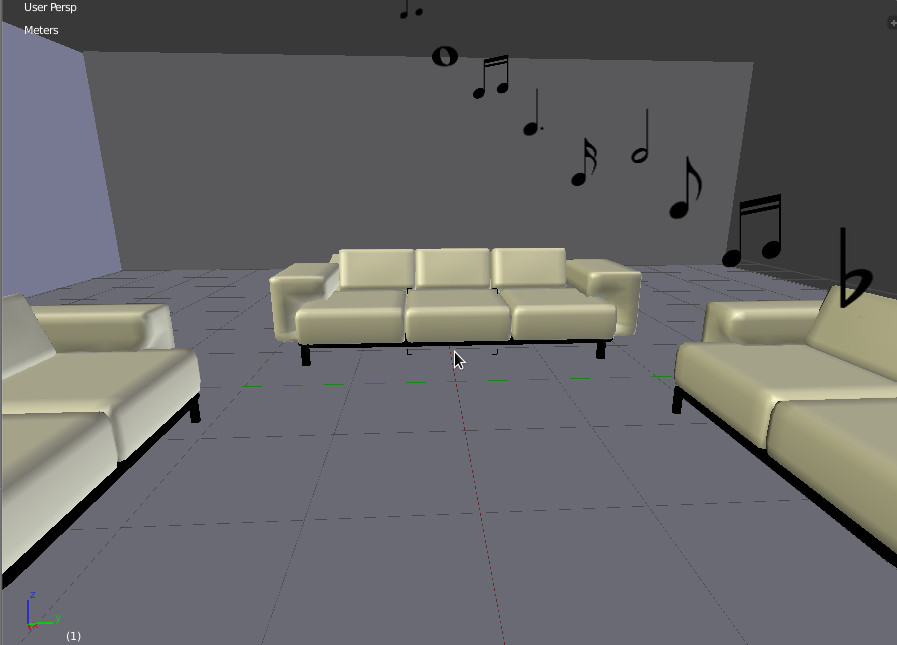
\includegraphics[width=90mm]{images/GD_basic.jpg}
\caption{Room with one object generating sound}
\label{sensorymockup1}
\end{figure}

\begin{figure}[H]
\centering
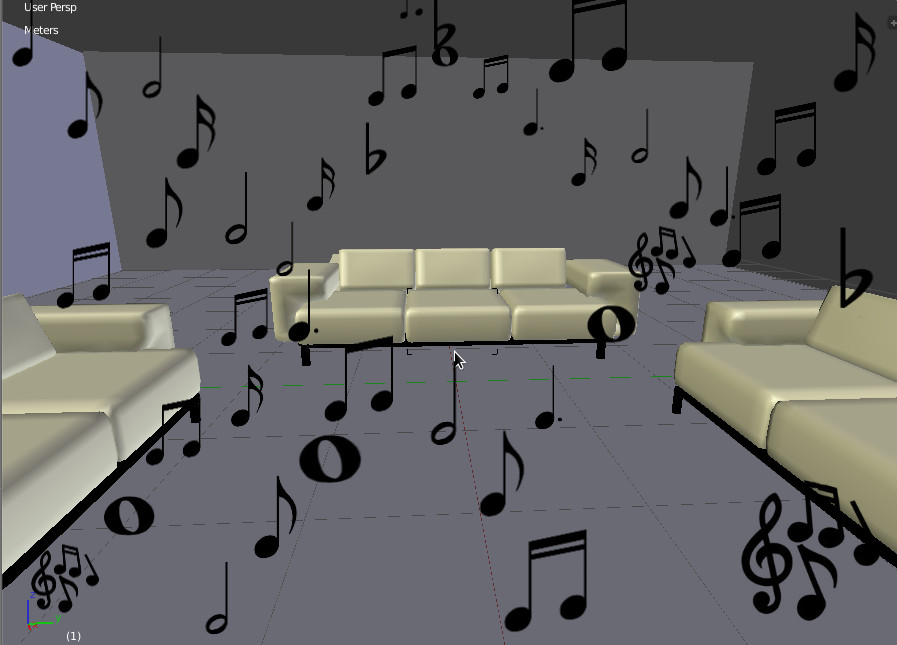
\includegraphics[width=90mm]{images/GD_moresound.jpg}
\caption{Effects of multiple objects creating sound}
\label{sensorymockup2}
\end{figure}

\begin{figure}[H]
\centering
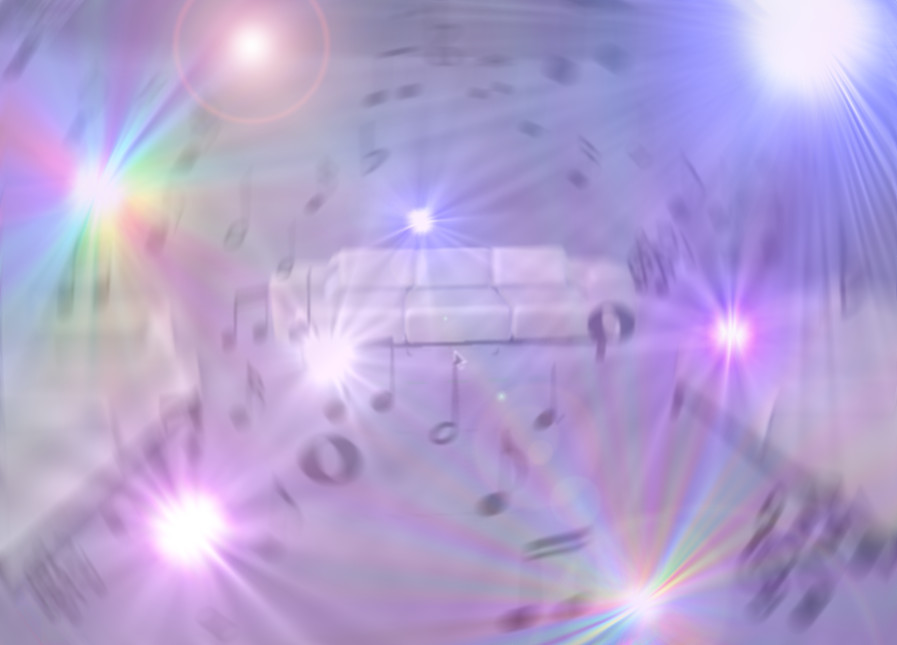
\includegraphics[width=90mm]{images/GD_overload.jpg}
\caption{Sensory overload. Lights have become brighter and environment is harder to see. Gaussian filter applied}
\label{sensoryoverloadmockup}
\end{figure}

2 of the 3 people interviewed specified that found the below image uncomfortable to view and was quite accurate. This demonstrates again that a sensory overload differs for each individual and indicates more should be consulted as 3 is a small sample. However, the projects core aim is to raise awareness of these problems rather than attempting to give an identical experience of having autism and thus this approach will be used unless feedback in the formative evaluation indicates changes are required. 

Sensory overloads will affect and be affected by the players contentment. If the player does not move away from troublesome objects quick enough, contentment will drop, which, if not addressed quick enough can lead to a meltdown. In addition, if contentment is low sensory overloads will occur quicker. 

\subsubsection{Special interests}
'Special interests' were chosen as a way to alleviate some of the difficulties within the environment and as a means to replenish energy or contentment. When engaging with a special interest, troublesome sounds will be reduced and if experiencing a sensory overload or meltdown the effects will subsidise. The special interest selected will be a Dinosaur toy which the user can interact with.

\subsubsection{Information processing delay}
Information processing delay was highlighted in interviews by a teacher as one of the main causes of meltdowns in school. When the user clicks on an object to interact or is expected to give a response, actions will be made harder to select by moving around. If the character has lower contentment the selections will move even quicker which should result in a greater delay from the player. Such delays could affect responses from other characters in the game. 

\subsection{Tool selection}
It was decided to use a game engine to allow time and focus to be directed onto the higher level concepts. Suitable game engine candidates were identified by looking at those highly rated on gamedev.net (extensive online resource for game developers), whilst taking some previous knowledge into account. Blender will be used as the modelling tool as it is freely available, powerful and well supported with lots of tutorials and documentation.

\subsubsection{Game engines}

** Put this in a table

\textbf{Unity}\\
Unity is one of the most popular game engines available with good support for models. Unfortunately the licence costs 1500 and the free version comes with limitations.

Advantages: popular game engine to use. Quick development with scripting. Phone app support.\\
Disadvantages: Interface heavy, limited to just scripting, costs, good computer required to run it efficiently.

\textbf{JMonkey}\\
JMonkey is a java 3d game engine that has been in development around for a few years. It has an extremely active and helpful community, allows complete customisation and holds little limitation being open source.

Advantages: Provides development environment with scene graph. Active community where you often get responses from developers themselves. Java is quick to develop in. Support for online use and phone apps. \\
Disadvantages: Java is not seen as the preferred language for graphics or games.

\textbf{Panda3D}\\
Originally created by Disney, Panda3D is an engine which can be used via python or C++ although support is mostly for python.

Advantages: Quick to develop for with a choice in language. Good community with lots of tools.\\
Disadvantages: No phone app and limited online support. Lack of documentation. 

\textbf{Ogre3D}\\
Ogre3d is primarily a graphics rendering engine and but it does have additional plugins such as 'physics' or drawing interfaces.

Advantages: Lots of modules and plugins. Powerful and used commercially. Active support community.\\
Disadvantages: Longer development process. Lack of tools such as a scene graph. No support for putting online.\\

JMonkey was chosen for its active community, development environment, because its programmed in Java and open-source. Although Java is not seen as the programming language of choice for graphics it allows quicker development than C++ counterparts. Unity allows very quick development with great results but the pro version would be required for some features, which is very expensive. As JMonkey is in Java it can be easily transferred to both an online game and an Android app which increases accessibility. Although an Android app may not be possible during the project timeline, converting the game to online should be straightforward. Finally there were no foreseen limitations with using JMonkey.

\subsubsection{Modelling tools}
For modelling there several options:
\begin{itemize}
\item Maya
\item 3DSMax
\item Blender
\item Sketchup
\end{itemize}

Blender was the primary 3D modelling tool of choice as it is free, open source, widely used for various game developers and professionals and the tool JMonkey is most built to accommodate.


\subsection{Character}
The character the user will play as. What difficulties they have/ what age they are.

\chapter{Formative evaluation}
- people mentioned that some of the effects were causing them sensory overloads

\chapter{Conclusions}

\section{Future work}

\begin{enumerate}
\item Occulus rift
\item Mind headset
\item Supporting others using system to build their own experiences
\item Research tool for how autism effects people in a different way.
\item Modelling people with autism and their difficulties and being able to see in what way the world effects them. 
\end{enumerate}

\begin{thebibliography}{9}

\bibitem{increasingprevalence}
Johnny L. Matson, Alison M. Kozlowski
The increasing prevalence of autism spectrum disorders. Research in Autism Spectrum Disorders(2011)

\bibitem{nas}
National autistic society. www.autism.org.uk

\bibitem{statsandfacts}
Ambitious about autism. www.ambitiousaboutautism

\bibitem{nasschool}
Make school make sense. Autism and education: the reality for families today. National Autistic Society, 

\bibitem{autismmisconception}
Autism misconceptions. NHS

\bibitem{olgab}
Sensory Perceptual Issues in Autism and Aspergers syndrome(2003). Bogdeshina, O

\bibitem{fears}
Unusual fears in children with autism(2012). Susan Dickerson Mayes, Susan L. Calhound, Richa Aggarwal, Courtner Baker, Santosh Mathapati, Sarah Molitoris, Rebeccas D. Mayes.

\bibitem{temperament}
Sensory correlates of difficult temperament characteristics in preschool children with autism(2012). I-Ching Chaung, Mei-Hui Tseng, Lu Lu, Jeng-Yi Shieh

\bibitem{bayes}
When the world becomes 'too real': a Bayesian explanation of autistic perception(2012). Elizabeth Pellicano and David Blurr.

\bibitem{williams1996}
Autism: An inside-out approach(1996). Williams, D

\bibitem{williams1994}
Somebody Somewhere: Breaking Free from the World of Autism(1994). Williams, D.

\bibitem{williams1992}
Nobody no-where(1992). Williams, D

\bibitem{sensory_leisure}
Sensory processing abilities and their relation to participation in leisure activities among children with high-functioning autism spectrum disorder. Hochhauser, M. Engel-Yeger, B.

\bibitem{sensory_toddlers}
Parent Reports of Sensory Symptoms in Toddlers with Autism and Those with Other Developmental Disorders. Sally J. Rogers, Susan Hepburn, Elizabeth Wehner

\bibitem{sensory_children}
Describing the sensory abnormalities of children and adults with autism(2007). Susan R. Leekam. Carmen Nieto. Sarah J. Libby. Lorna wing. Judith gould. 

\bibitem{sensory_perceptual}
Sensory integration and the perceptual experience of persons with autism(2006). Grace Iarocci. John McDonald.

\bibitem{rss_cognitive}
Restricted and Repetitive Behaviours, Sensory Processing and Cognitive Style in Children with Autism Spectrum Disorders(2009). Yu-Han Chen, Jacqui Rodgers, Helen McConachie.

\bibitem{rrsyouth}
Restricted and repetitive behaviours and psychiatric symptoms in youth with autism spectrum disorders(2013) Elizabeth A. Stratic, Luc Lecavlier.

\bibitem{rrs_sensory}
Is there a relationship between restricted, repetitive, sterotyped behaviours and interests and abnormal sensory response in children with autism spectrum disorders?(2008). Robin L. Gabriels, John A. Agnew, Lucy Jane Miller, Jane Gralla, Juliet P. Dinkins, Elizabeth Hooks.

\bibitem{aspieway}
"It’s like you are just a spectator in this thing": Experiencing social life the 'aspie' way(2008). Sara Ryan, Ulla Raisanen

\bibitem{dd}
Disability awareness: Beyond the day: http://www.serviceandinclusion.org/index.php?page=simulations. Danielle Dreilinger

\bibitem{autism_awareness}
Awareness and knowledge of autism and autism interventions: A general population survey. Karola Dillenburger(2013). Julie Ann Jordan, Lyn McKerr, Paula Devine, Mickey Keenan

\bibitem{teachersinclusion}
Factors relating to education professionals' classroom practices for the inclusion of students with ASD. Matthew J Segall, Jonathon M. Campbell. 

\bibitem{meltdowns_goingout}
'Meltdowns', surveillance and managing emotions: going out with children with autism(2010). Sara Ryan.

\bibitem{sensory_overview}
Sensory issues in Autism(2007). East sussex county council. 

\bibitem{rss_anxiety}
Relations amoung restricted and repetitive behaviours, anxiety and sensory features in children with autism spectrum disorders(2004)

\end{thebibliography}

\end{document}